\begin{figure}[!b]
    \centering
    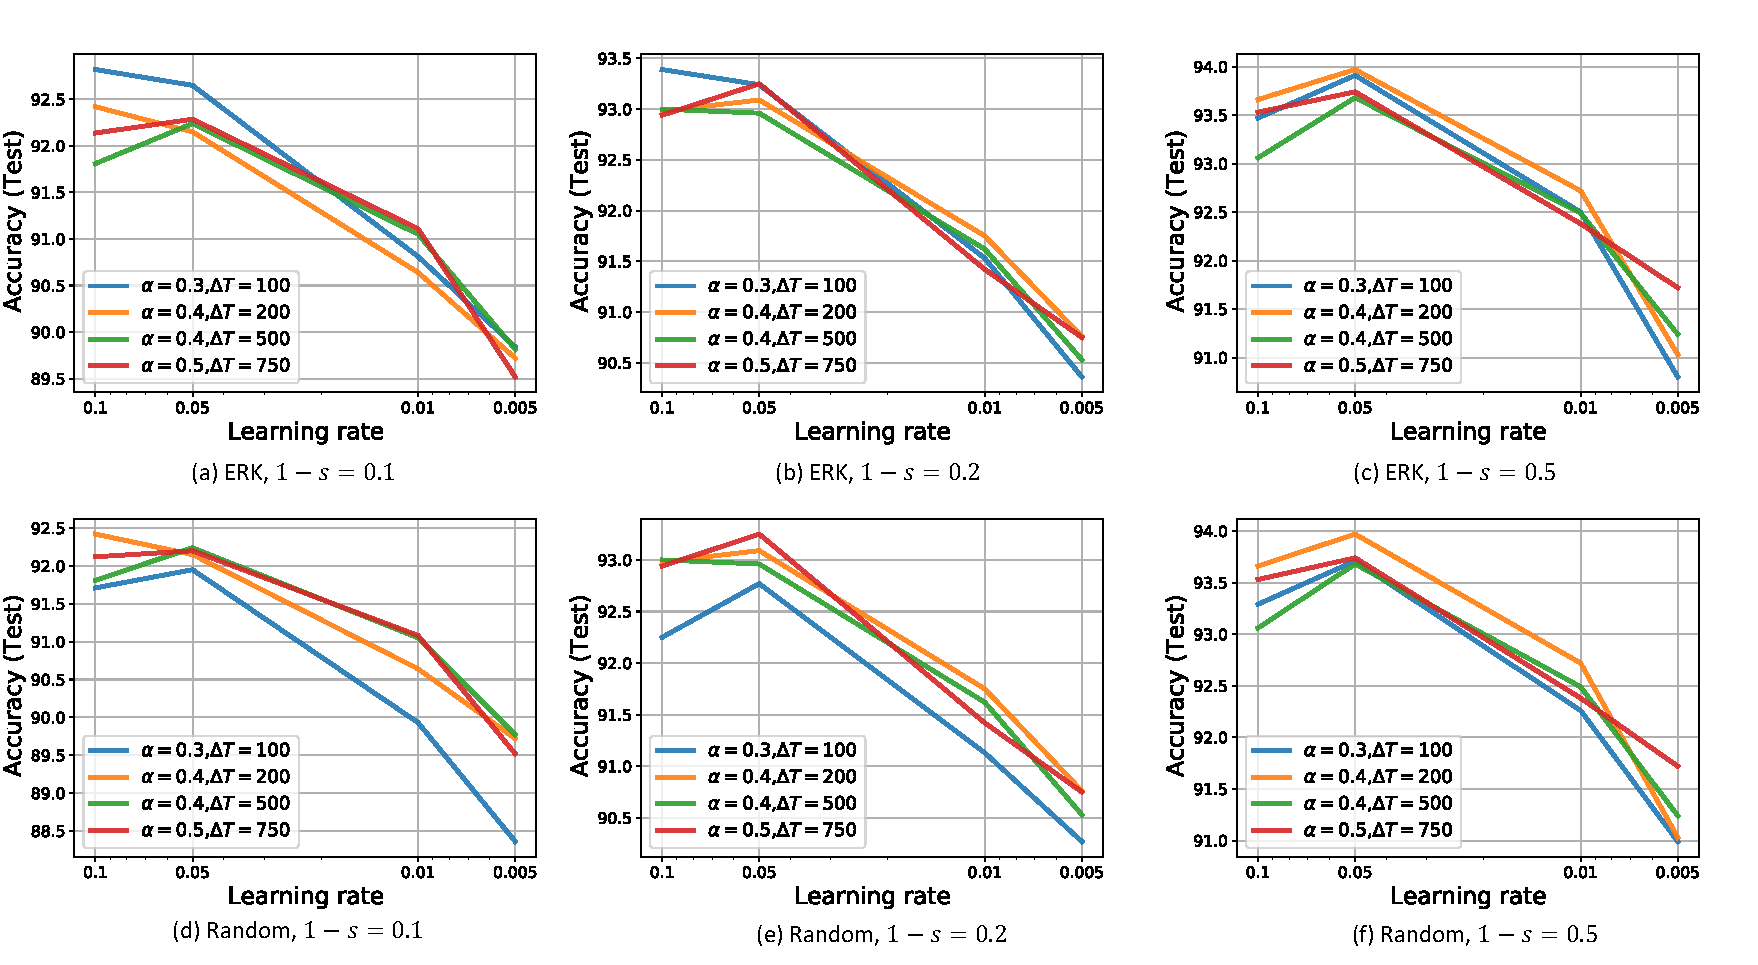
\includegraphics[width=\textwidth]{../openreview/figs/lr_sweep.pdf}
    \captionsetup{aboveskip=\figureaboveskip,belowskip=\figurebelowskip}
    \caption{\textbf{Learning Rate vs Sparsity on CIFAR-10.} Runs using a learning rate $> 0.1$ do not converge and are not plotted here. There is little benefit in tuning the learning rate for each sparsity, and $0.1, 0.05$ are good choices overall.}
    \label{fig:lr-sweep}
\end{figure}